\documentclass[a4paper, 12pt]{article}

%%%%%%%%%%%%%%%%%%%%%%%%%%%%%%% PACKAGES %%%%%%%%%%%%%%%%%%%%%%%%%%%%%%%
% Math-related things
\usepackage{amsmath}
\usepackage{amssymb}
\usepackage{amsthm}
% Italian spelling
\usepackage[italian]{babel}
% Accenti e caratteri speciali
\usepackage[utf8]{inputenc}
% Margini e grafica della pagina
\usepackage[top=2cm, bottom=2cm, left=2cm, right=2cm]{geometry}
\usepackage{fancyhdr}
% Tabelle
\usepackage{tabularx}
% Graphs and Images handling
\usepackage{graphicx}
\usepackage{svg}
% Programming languages support
\usepackage{minted}
% Hypertext references
\usepackage{hyperref}
% Citations
\usepackage{epigraph}

% Title Page
\title{TasteIt - Progetto di Ingegneria Informatica}
\author{
	Paolo Pertino [10729600]
	\href{mailto:paolo.pertino@mail.polimi.it}{paolo.pertino@mail.polimi.it} \\
	Supervisionato da Professor Giovanni Agosta
	\href{mailto:giovanni.agosta@polimi.it}{giovanni.agosta@polimi.it}
} 

% Contents page settings
\renewcommand*\contentsname{Indice}
\setcounter{tocdepth}{3}

\newcommand{\quantities}[1]{%
	\begin{tabular}{@{}c@{}}\strut#1\strut\end{tabular}%
}

% General page settings
\pagestyle{fancy}
\fancyhf{}
\rhead{\leftmark}
\lhead{TasteIt - Progetto di Ingegneria Informatica}
\cfoot{\thepage}

% Hyperrefs setup
\hypersetup{
	colorlinks=true,
	linkcolor=[rgb]{0.996,0.396,0.090196}, %254 101 23
	filecolor=magenta,      
	urlcolor=[rgb]{0.72156862745,0.0078431372549,0.00392156862745},
	citecolor=[rgb]{0.517647,0.0156862745,0.0117647},
	pdftitle={TasteIt - Progetto di Ingegneria Informatica},
	pdfpagemode=FullScreen,
}

\begin{document}
	\pagenumbering{gobble}
	\date{\today}
	\maketitle
	
	\begin{figure}[h!]
		\centering
		
\includegraphics[scale=0.35]{tasteitIntro.png}
	\end{figure}

	\newpage
	\pagenumbering{arabic}
	
	\tableofcontents
	
	\newpage
	
	\section{Introduzione}
	\paragraph{}
	TasteIt è un bot Telegram che si propone di aiutare gli utenti a effettuare una ricerca del ristorante in cui consumare un pasto, in base alle loro esigenze in termini di ciò che vogliono mangiare, orario, prezzo e distanza. La ricerca può aver inizio a partire dalla propria posizione, oppure dal nome di una località, piazza o via di interesse.\\
	Infine, la semplice operazione di ricerca è stata corredata dalla possibilità di creare liste dei preferiti, interattività della conversazione nei gruppi con possibilità di creare sondaggi ed è inoltre fornito un supporto per diverse lingue (attualmente sono implementate solo Italiano e Inglese).
	
	\subsection{Obiettivi}
	\paragraph{}
	Come anticipato nel paragrafo precedente, TasteIt si propone di essere una valida interfaccia per i servizi offerti da Google Maps in termini di ricerca di ristoranti. Per questo motivo, di seguito elenchiamo i principali obiettivi preposti:
	\begin{itemize}
		\item \textbf{Ricerca personalizzata}
		
		Offrire una ricerca personalizzata del ristornate in cui consumare il proprio pasto, in termini di cibo desiderato, orario di apertura, fascia di prezzo, posizione iniziale di ricerca e preferenze relative alla distanza massima che si vuole percorrere (2 filtri di default per indicare la volontà di sopraggiungere al locale a piedi o in macchina).
		
		\item \textbf{Informazioni del ristorante}
		
		Fornire inizialmente delle informazioni riassuntive (che possiamo assumere essere valutazione complessiva e numero di recensioni) che permettano all'utente di scegliere un ristorante e successivamente, sotto richiesta dello stesso, mostrare informazioni più dettagliate, comprendenti anche indirizzo, numero di telefono, sito web (se presente) e recensioni degli utenti.
		
		\item \textbf{Gestione preferiti}
		
		Offrire la possibilità ad utenti e gruppi di salvare i ristoranti di interesse in liste dei preferiti, consultabili in autonomia in qualsiasi momento.
		
		\item \textbf{Interattività nei gruppi}
		
		Rendere interattivo ed utilizzabile il bot nei gruppi, in modo tale da essere uno strumento effettivamente utile per coordinare l'organizzazione di più persone. A tal proposito, solamente nei gruppi, a valle di una ricerca effettuata, permettere la decisione attraverso sondaggi.
		
		\item \textbf{Persistenza dei dati}
		
		I dati principali dell'utente o di un gruppo, quali lingua ed impostazioni relative ai filtri di distanza massima, devono essere persistenti e non relegati alla singola conversazione.
		
		\item \textbf{Multilingua}
		
		Permettere la personalizzazione della lingua \textit{"parlata"} dal bot. Offrire di default Italiano e Inglese.
	\end{itemize}

	\newpage
	\subsection{Requisiti}
	\paragraph{}
	Per far fronte agli obiettivi dichiarati nella sezione precedente, TasteIt deve soddisfare i seguenti requisiti:
	\begin{itemize}
		\item \textbf{Parametrizzazione della ricerca}
		
		Permettere all'utente di personalizzare la propria ricerca, fornendogli la possibilità di modificare tutti i parametri che caratterizzano la stessa (cibo desiderato, fascia di prezzo, orario, metodo di raggiungimento) nella fase che la precede.
		
		\item \textbf{Richiesta e gestione delle informazioni}
		
		Per limitare i costi delle Places API è necessario fare richiesta, \textbf{nel momento opportuno}, delle sole informazioni di interesse. É pertanto necessario prevedere fasi distinte tra visualizzazione della lista dei ristoranti della zona di ricerca ed informazioni dettagliate di un singolo locale.
		
		\item \textbf{Persistenza e gestione dei dati}
		
		Costruire un'apposita base di dati che permetta di salvare le informazioni relative agli utenti e ai gruppi, come lingua desiderata e liste dei preferiti, in modo tale che esse siano consultabili e modificabili in qualsiasi momento.
		
		\item \textbf{Compatibilità con i gruppi}
		
		Fornire la compatibilità delle conversazioni, di default disponibili in chat privata, anche nei gruppi, prevedendo l'interazione del bot con molteplici agenti in una stessa conversazione. Per agevolare l'operazione di scelta di un ristorante, permettere la creazione di sondaggi tra i ristoranti appartenenti alla lista che si sta visualizzando.
	\end{itemize}
	
	\newpage
	\subsection{Installazione}
	\paragraph{}
	Per poter avviare il bot è necessario avere Python 3.x \cite{python_installation} installato sul proprio dispositivo.\\
	Attraverso il packet manager \textit{pip} installare i requirements elencati nel file \textit{requirements.txt}, recandosi nella directory principale del progetto (\textit{./TasteIt}) e digitando il comando:
	\begin{minted}{bash}
		$ pip install -r requirements.txt
	\end{minted}
\subsubsection{Configurazione Telegram}
	\paragraph{}
	Successivamente è necessario creare un bot attraverso \textit{@BotFather} ed ottenere la API key associata \cite{telegram_bot_creation}.\\
	Creare dunque un file \textit{.env} all'interno della cartella \textit{/src} in cui inserire la chiave appena generata con il seguente formato:
	\begin{minted}{bash}
		TELEGRAM_KEY=la_tua_chiave
	\end{minted}
	\paragraph{}
	Inoltre, collegarsi nella chat di \textit{@chatIDrobot} e premere \textit{Avvia} per ottenere informazioni riguardanti la propria chat. Copiare il numero che segue la dicitura \textit{chat\_id} ed inserirlo nel file \textit{.env} con il formato seguente:
	\begin{minted}{bash}
		TELEGRAM_DEVELOPER_CHAT_ID_KEY=chat_id_copiato
	\end{minted}
	In questo modo quando un errore inaspettato verrà riscontrato da un utente, il bot provvederà in automatico a segnalare lo sviluppatore.
	\paragraph{}
	La configurazione dei parametri inerenti Telegram è ora completata.
	
	\subsubsection{Configurazione Google}
	\paragraph{}
	Dal momento che il funzionamento del bot è relegato all'utilizzo dei servizi offerti da Google, attraverso le \textit{Places API}, è necessario registrare un account su \textit{Google Cloud Services} e fare richiesta per l'abilitazione di una key per le suddette API \cite{places_api_key_registration}.
	Una volta ottenuta le chiave, inserirla all'interno del file \textit{.env} con il formato che segue:
	\begin{minted}{bash}
		GOOGLE_PLACES_KEY=la_tua_google_api_key
	\end{minted}
	
	\subsubsection{Configurazione Mapbox}
	Infine, per usufruire delle complete funzionalità è necessario attivare un account Mapbox\cite{mapbox_api} e generare un'ulteriore API Key per tale servizio.\\
	\begin{minted}{bash}
		MAPBOX_KEY=la_tua_mapbox_api_key
	\end{minted}
	In alternativa è possibile installare sulla propria macchina un server OSRM \cite{osrm} che gestisca la parte di backend per le informazioni sul percorso da compiere.
	\paragraph{}
	Terminato questo passaggio, il bot è pronto per essere avviato. Digitare dunque il comando:
	\begin{minted}{bash}
		$ py ./main.py
	\end{minted}
	per avviare l'applicativo.
	
	\newpage
	\subsubsection{Permessi per i gruppi}
	\paragraph{}
	Se si vuole aggiungere TasteIt ad un gruppo, assicurarsi di fornirgli i seguenti permessi da amministratore:
	\begin{figure}[h!]
		\centering
		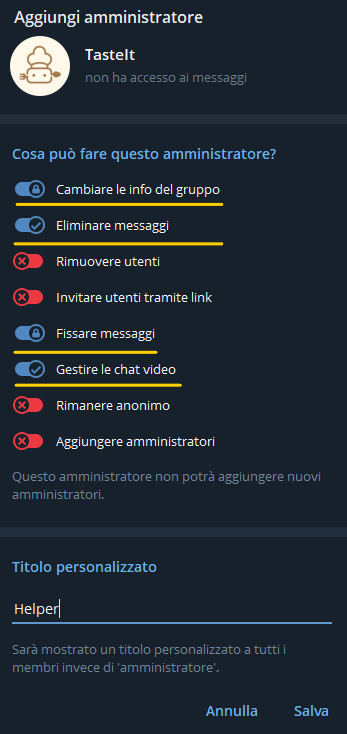
\includegraphics[scale=1.1]{adminPermissions.png}
		\caption{Permessi da assegnare a TasteIt nei gruppi}
	\end{figure}
	
	\newpage
	% Lista di funzionalità
	\section{Funzionalità TasteIt}
	Di seguito elenchiamo le funzionalità offerte dal bot ed i comandi necessari per l'interazine.
	\begin{itemize}
		\item \textit{/start} - Avvia il bot mostrando un messaggio di benvenuto all'utente.
		\item \textit{/help} - Permette la visualizzazione di tutti i comandi disponibili.
		\item \textit{/settings} - Permette la modifica di alcuni parametri di ricerca.
		\item \textit{/lang} - Permette il cambio di lingua. Esso impatterà sia sui messaggi di servizio sia sugli effettivi risultati di ricerca.
		\item \textit{/cerca} - Introduce la conversazione per iniziare la ricerca di un ristorante.
		\item \textit{/preferiti} - Mostra all'utente (o al gruppo) le sue liste preferiti.
		\item \textit{/annulla} - Annulla l'operazione corrente.
	\end{itemize}
	
	\subsection{/lang - Modifica lingua}
	\paragraph{}
	Digitando il comando \textit{/lang} è possibile modificare la lingua con cui interagire con il bot. Quest'ultimo invierà un messaggio con allegato una tastiera contenente le lingue disponibili (di default soltanto Italiano ed Inglese).
	
	\begin{figure}[h!]
		\centering
		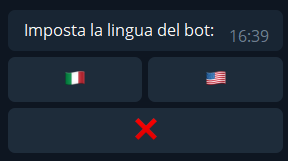
\includegraphics[scale=1.1]{langCommand.png}
		\caption{Risposta al comando /lang}
	\end{figure}

	Selezionando una delle bandiere, la lingua muterà in quella selezionata ed i dati verranno anche aggiornati nel database.
	
	\subsection{/settings - Modifica dei filtri sul raggio di ricerca}
	\paragraph{}
	Attraverso il comando \textit{/settings} è possibile modificare i parametri di default relativi alla massima distanza percorribile sia a piedi sia in macchina (di default a piedi 0.5 km e in macchina 10 km).\\
	Tali nuove informazioni saranno salvate nel database in modo tale da essere utilizzate come limite massimo di lunghezza del percorso da compiere quando si effettua un'operazione di ricerca di un ristorante.
	\newpage
	\begin{figure}[h]
		\centering
		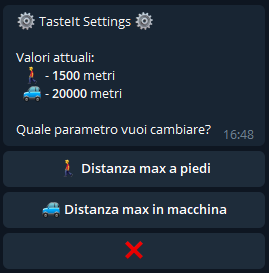
\includegraphics[scale=0.9]{settingsCommand.png}
		\caption{Risposta al comando /settings}
	\end{figure}
	\paragraph{}
	Cliccando il bottone \textit{Distanza max a piedi} o \textit{Distanza max in macchina} sarà successivamente possibile scegliere un valore compreso tra 1 e 50'000 per indicare il nuovo raggio di ricerca da settare come valore di default (in metri) per gli spostamenti a piedi o in macchina.\\
	
	\subsection{/cerca - Ricerca dei ristoranti}
	\paragraph{}
	A seguito del comando \textit{/cerca} inizierà la conversazione che gestisce l'intera fase di ricerca di un ristorante. La procedura è interamente guidata ed è articolata in diversi passi, di cui di seguito presentiamo una breve descrizione e delle immagini prese dalla conversazione stessa.
	
	\begin{enumerate}
		\item \textbf{Richiesta della posizione}
		
		Il primo step richiede all'utente di inserire la posizione da cui far iniziare la ricerca. Essa può essere specificata manualmente fornendo il nome di una località, via, piazza, etc... oppure inviando la propria posizione attuale utilizzando la funzionalità nativa di telegram.
		
		\begin{figure}[!htb]
			\begin{minipage}{0.45\textwidth}
				\centering
				
\includegraphics[width=\linewidth]{cercaCommand_startingPoseByName.png}
				\caption{Posizione iniziale da nome}
			\end{minipage}\hfill
			\begin{minipage}{0.45\textwidth}
				\centering
				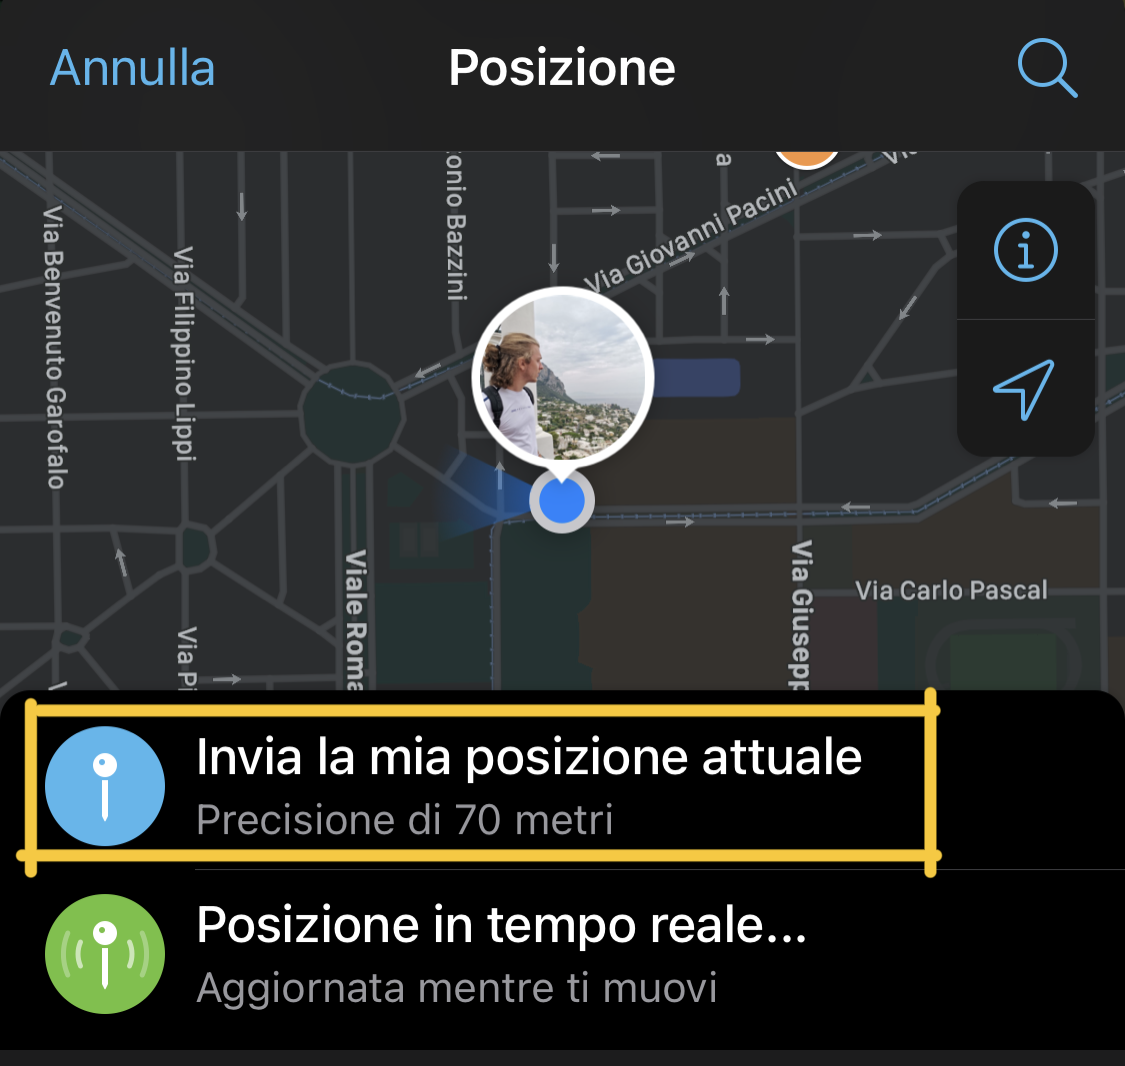
\includegraphics[width=\linewidth]{cercaCommand_startingPoseByCurrentPosition.png}
				\caption{Posizione iniziale da posizione attuale}
			\end{minipage}
		\end{figure}
	
		\item \textbf{Richiesta del tipo di cibo}
		
		Il secondo step prevede l'inserimento da parte dell'utente di ciò che vuole mangiare.
		\begin{figure}[!htb]
			\centering
			
\includegraphics[scale=0.9]{cercaCommand_foodChoice.png}
			\caption{Scelta del cibo}
		\end{figure}
	
		\item \textbf{Messaggio di recap}
		
		Il terzo step consiste nella revisione di tutti i parametri con cui verrà effettuata la ricerca.
		Al messaggio di recap vengono affissi dei bottoni che permettono di modificare tali parametri. Nello specifico è possibile:
		\begin{enumerate}
			\item modificare la preferenza riguardante il cibo;
			\item includere nella ricerca i ristoranti che da orario sono, al momento della stessa, chiusi oppure escluderli e visualizzare soltanto quelli aperti;
			\item modificare la fascia di prezzo;
			\item scegliere se sopraggiungere al locale a piedi oppure in macchina;
		\end{enumerate}
		\begin{figure}[!htb]
			\centering
			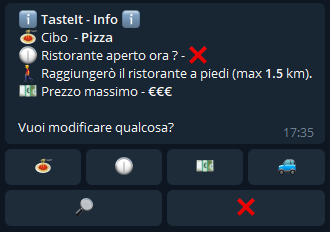
\includegraphics[scale=0.9]{cercaCommand_recapMsg.png}
			\caption{Messaggio di recap}
		\end{figure}
		Premendo la lente di ingrandimento avrà dunque inizio la ricerca con i parametri specificati.
		
		\item \textbf{Visualizzazione lista dei ristoranti trovati}
		
		Dopo una breve attesa, verrà inviato un messaggio a cui è affissa una tastiera per scorrere i ristoranti estratti che soddisfano le caratteristiche specificate negli stage precedenti. Per ogni locale sono mostrate poche informazioni, quali nome, distanza e tempo di percorrenza del tragitto per sopraggiungervi, valutazione media degli utenti e numero totale di recensioni. 
			
		\newpage
		\begin{figure}[!htb]
			\begin{minipage}{0.35\textwidth}
				\centering
				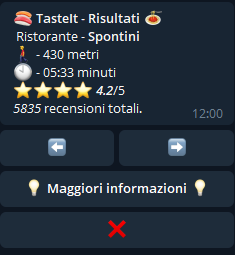
\includegraphics[width=\linewidth]{cercaCommand_generalRestaurantInfoList.png}
				\caption{Lista di ristoranti}
			\end{minipage}\hfill
			\begin{minipage}{0.35\textwidth}
				\centering
				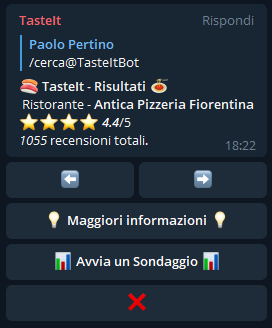
\includegraphics[width=\linewidth]{cercaCommand_generalRestaurantInfoListGroups.png}
				\caption{Lista dei ristoranti nei gruppi}
			\end{minipage}
		\end{figure}
	
		\item \textbf{Informazioni dettagliate}
		
		Cliccando il pulsante \textit{"Maggiori informazioni"} verranno effettivamente mostrate info più dettagliate sul ristorante scelto.
		\begin{figure}[!htb]
			\centering
			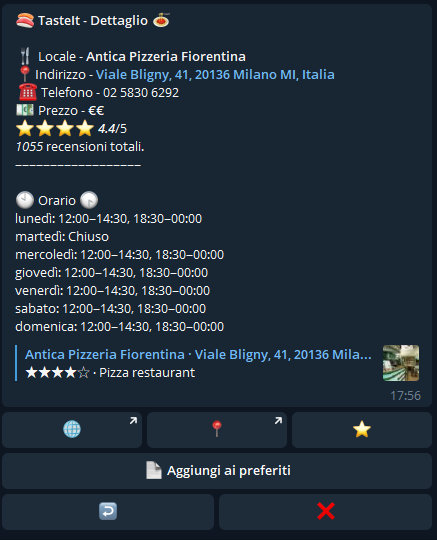
\includegraphics[scale=0.78]{cercaCommand_detailedInfo.png}
			\caption{Lista di ristoranti}
		\end{figure}
	\newpage
	\paragraph{}
	I bottoni legati al messaggio permettono rispettivamente di visitare il sito web (se presente), aprire Google Maps alla posizione del ristorante per ottenere indicazioni, visualizzare le recensioni e aggiungere il locale ad una lista dei preferiti.
	
	\item \textbf{Recensioni}
	
	Cliccando la stella è possibile visualizzare le recensioni del ristorante, se presenti:
	\begin{figure}[!htb]
		\centering
		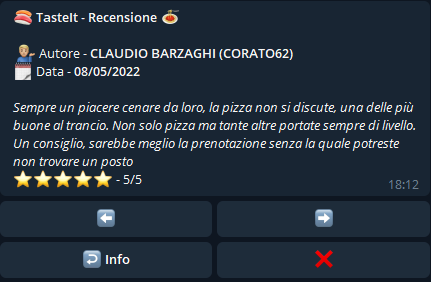
\includegraphics[scale=0.9]{cercaCommand_viewReviews.png}
		\caption{Visualizzazione delle recensioni}
	\end{figure}
	\paragraph{}
	Cliccando sulle frecce poste sul lato superiore della tastiera è possibile scorrere le recensioni.
	
	\item \textbf{Aggiungi ai preferiti}
	
	Invece, con un tap sul bottone \textit{Aggiungi ai preferiti} è infine possibile aggiungere il ristorante di cui si stanno visualizzando le informazioni dettagliate ad una lista dei preferiti. É possibile scegliere sia una lista già esistente, sia crearne una nuova come è possibile notare in figura.
	\begin{figure}[!htb]
		\centering
		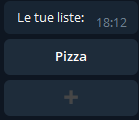
\includegraphics[scale=0.9]{cercaCommand_addToFavorites.png}
		\caption{Aggiungi ai preferiti}
	\end{figure}
	\paragraph{}	
	\end{enumerate}
	
	\newpage
	\subsection{/preferiti - Lista dei preferiti}
	\paragraph{}
	Utilizzando il comando \textit{/preferiti} inizia la conversazione che gestisce la visualizzazione delle proprie liste dei preferiti, se presenti, e del loro aggiornamento (cancellazione della lista e rimozione di ristoranti).
	
	\begin{figure}[!htb]
		\begin{minipage}{0.45\textwidth}
			\centering
			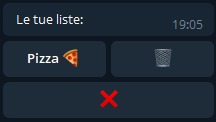
\includegraphics[width=\linewidth]{preferitiCommand_listOfLists.png}
			\caption{Le tue liste}
		\end{minipage}\hfill
		\begin{minipage}{0.45\textwidth}
			\centering
			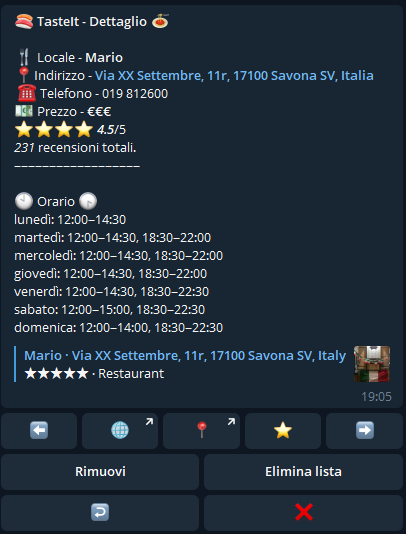
\includegraphics[width=\linewidth]{preferitiCommand_listContent.png}
			\caption{Contenuto della lista}
		\end{minipage}
	\end{figure}

	\paragraph{}
	Come è possibile notare, vengono direttamente mostrate le informazioni dettagliate dei ristoranti presenti nelle liste preferiti. I comandi fruibili attraverso i bottoni, inoltre, sono i medesimi visti per la fase di ricerca e comprendono quindi la visualizzazione del sito web, indicazioni su \textit{Google Maps} e recensioni del locale.\\
	Nei gruppi è inoltre possibile avviare un sondaggio con i ristoranti contenuti nella lista che si sta visualizzando.
	
	
	\newpage
	% Architettura
	\section{Architettura}
	Nella sezione corrente viene resa esplicita l'architettura dell'applicativo. Nello specifico vengono presentate ed analizzate:
	\begin{itemize}
		\item Struttura del database.
		\item Oggetti custom creati per gestire le liste di ristoranti.
		\item Macchine a stati rappresentanti le conversazioni.
	\end{itemize}
	\subsection{Database}
	Nella Figura \ref{fig:ER_image} è stato riportato il diagramma ER rappresentante la semplice struttura del database.
	\begin{figure}[h!]
		\centering
		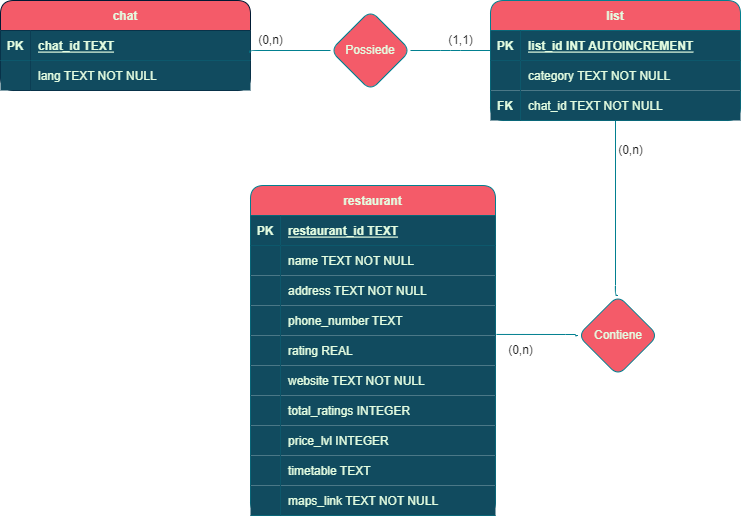
\includegraphics[scale=0.62]{tasteItDb.png}
		\caption{Schema ER Database TasteIt}
		\label{fig:ER_image}
	\end{figure}
	\paragraph{}
	La relazione \textit{'Contiene'} è stata successivamente trasformata in una tabella ponte chiamata \textit{restaurant\_for\_list}.
	Pertanto, riportiamo di seguito lo schema logico dedotto dalla progettazione concettuale effettuata:\\
	chat(\textbf{chat\_id}, lang, preferred\_distance\_on\_foot, preferred\_distance\_by\_car)\\
	restaurant(\textbf{restaurant\_id}, name, address, phone\_number, rating, website, total\_ratings, price\_lvl, timetable, maps\_link)\\
	list(\textbf{list\_id}, category, chat\_id)\\
	restaurant\_for\_list(\textbf{list\_id, chat\_id})\\
	list.chat\_id $\rightarrow$ chat.chat\_id\\
	restaurant\_for\_list.list\_id $\rightarrow$ list.list\_id\\
	restaurant\_for\_list.chat\_id $\rightarrow$ chat.chat\_id
	
	\subsection{Class Diagram}
	\paragraph{}
	Di seguito riportiamo inoltre un class diagram degli oggetti ausiliari creati ed utilizzati ai fini del progetto.\\
	\begin{figure}[h]
		\centering
		\def\svgwidth{\columnwidth}
		\resizebox{\linewidth}{!}{\input{{tasteit_class_diagram.pdf_tex}}}
		\caption{TasteIt - Class Diagram}
		\label{fig:class_diagram}
	\end{figure}
	\paragraph{}
	Segue una breve descrizione del contenuto della Figura \ref{fig:class_diagram}:
	\begin{itemize}
		\item \textit{Service} enumerazione rappresentante i servizi per cui è disponibile una API key;
		\item \textit{ApiKey} rappresenta la chiave stessa. Il metodo \textit{value} cerca la key del servizio specificato all'interno del file \textit{.env} o tra le variabili d'ambiente del sistema;
		\item \textit{ResearchInfo} rappresenta le informazioni preliminari utili per effettuare una ricerca di un ristorante;
		\item \textit{GeneralPlace} contiene le informazioni relative alla posizione di un determinato luogo;
		\item \textit{DoublyCircularArrayList} classe astratta rappresentante una doppia lista circolare\cite{circularDoublyLinkedList} (differente dalla versione linked, in quanto i nodi non sono effettivamente linkati tra loro);
		\item \textit{Restaurant} rappresenta un ristorante e tutte le sue informazioni (nome, latitudine, longitudine, 'costosità', valutazione media degli utenti, numero totale di recensioni, orario settimanale, indirizzo, sito web, link a google maps e numero di telefono);
		\item \textit{Rating} rappresenta una recensione (autore, valutazione, contenuto e data);
		\item \textit{RestaurantsList} implementazione di DoublyCircularArrayList rappresentante una lista di ristoranti;
		\item \textit{RatingsList} implementazione di DoublyCircularArrayList rappresentante una lista di recensioni;
		\item \textit{ListIterator} iteratore per le liste sopra descritte, il quale le rende iterabili da inizio a fine;
		\item \textit{FavoriteList} rappresenta una lista preferiti (id, categoria e ristoranti in essa contenuti);
	\end{itemize}

	\subsection{Conversazioni - Macchine a stati}
	\paragraph{}
	In questa sezione verranno presentate le macchine a stati schematizzanti le conversazioni offerte dal bot e gli eventi che scatenano i cambiamenti di stato.
	\subsubsection{Modifica della lingua}
	\paragraph{}
	La conversazione più semplice: in risposta al comando \textit{/lang} viene invocata la funzione \textit{setLanguage()} che presenta all'utente il messaggio con la tastiera per scegliere la lingua da utilizzare.\\
	\begin{figure}[h!]
		\centering
		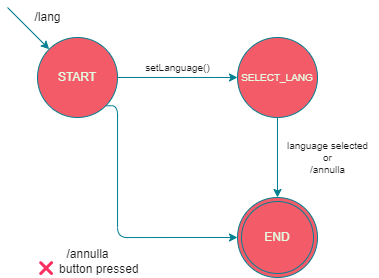
\includegraphics[scale=0.7]{TasteIt_Lang_StateMachine.png}
		\caption{/lang - State Machine}
		\label{fig:LangStateMachine}
	\end{figure}
	
	\newpage
	\subsubsection{Ricerca ristorante}
	\paragraph{}
	Risponde alla richiesta effettuata con il comando \textit{/cerca} e gestisce l'intera conversazione di ricerca dei ristoranti e visualizzazione dei risultati.\\
	\begin{figure}[h!]
		\centering
		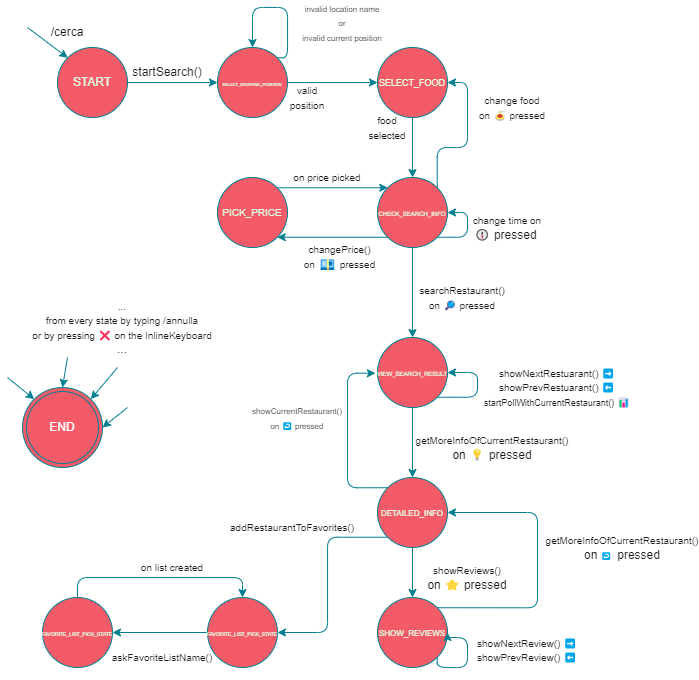
\includegraphics[scale=0.6]{TasteIt_Cerca_StateMachine.png}
		\caption{/cerca - State Machine}
		\label{fig:CercaStateMachine}
	\end{figure}
	
	\newpage
	\subsubsection{Visualizza lista preferiti}
	\paragraph{}
	Risponde al comando \textit{/preferiti}. Gestisce l'intera conversazione che permette di visualizzare e modificare le proprie liste dei preferiti.\\
	\begin{figure}[h!]
		\centering
		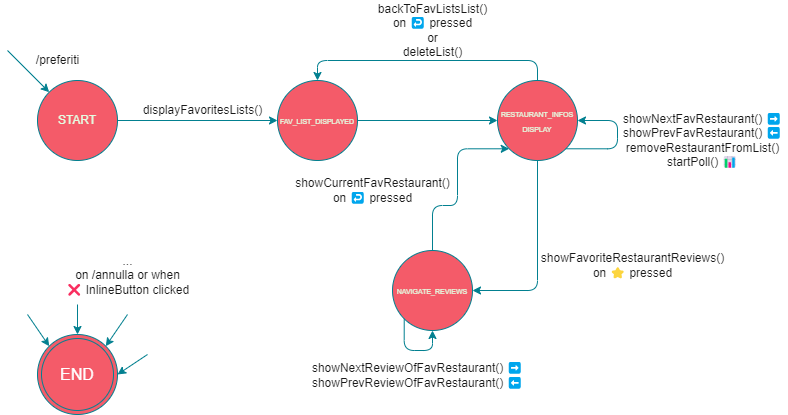
\includegraphics[scale=0.6]{TasteIt_Preferiti_StateMachine.png}
		\caption{/preferiti - State Machine}
		\label{fig:PreferitiStateMachine}
	\end{figure}

	\subsubsection{Modifica impostazioni}
	\paragraph{}
	Risponde al comando \textit{/settings}. Gestisce la conversazione che permette all'utente di modificare i suoi parametri di default relativi alla distanza massima percorribile quando viene effettuata una ricerca.
	\begin{figure}[h!]
		\centering
		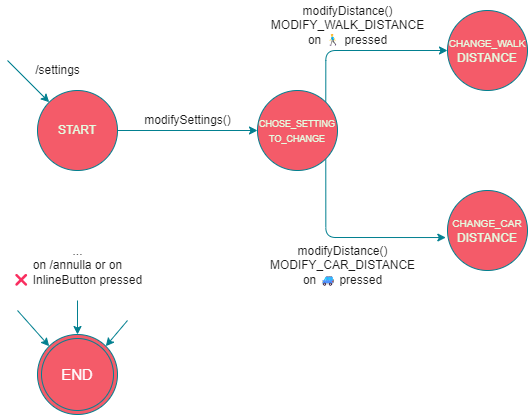
\includegraphics[scale=0.57]{TasteIt_Settings_StateMachine.png}
		\caption{/settings - State Machine}
		\label{fig:SettingsStateMachine}
	\end{figure}

	% Strumenti usati
	\newpage
	\section{Strumenti utilizzati}
	Nella seguente sezione verranno indicati i principali strumenti di sviluppo utilizzati:\\
	\begin{itemize}
		\setlength{\parskip}{0pt}
		\setlength{\parsep}{0pt}
		
		\item \emph{Visual Studio Code} - Principale IDE utilizzato.
		\item \emph{python-telegram-bot} - Wrapper python usato per interfacciarsi con le API di Telegram.
		\item \emph{Places API} - Google Maps API; gestiscono l'operazione di ricerca dei ristoranti.
		\item \emph{Mapbox} - Informazioni riguardo al tragitto da percorrere per giungere a destinazione.
		\item \emph{SQLite3} - modulo per interagire con le API dell'omonima libreria SQLite, utilizzata per creare e gestire databases in locale.
		\item \emph{Raspberry PI 4} - Hosting del bot e gestione del database.
		\item \emph{AstahUML} - Creazione di diagrammi UML.
		\item \emph{GitKraken} - Git GUI per visualizzare il workflow di sviluppo ed utilizzare efficientemente Git.
		\item \emph{TEXStudio} - Gestione e aggiornamento del report.
	\end{itemize}
	% Bibliografia
	\newpage
	\begin{thebibliography}{99}
		\bibitem{python_installation}
		\href{https://www.python.org/downloads/}{Python Download \& Installation}
		
		\bibitem{telegram_bot_creation}
		\href{https://sendpulse.com/knowledge-base/chatbot/create-telegram-chatbot}{Create a Telegram bot}
		
		\bibitem{places_api_key_registration}
		\href{https://developers.google.com/maps/documentation/places/web-service/get-api-key}{Google Cloud Platform - Places API Key}
		
		\bibitem{mapbox_api}
		\href{https://www.mapbox.com/}{Mapbox Website}
		
		\bibitem{osrm}
		\href{https://github.com/Project-OSRM/osrm-backend}{OSRM-backend}
		
		\bibitem{circularDoublyLinkedList}
		\href{https://pythonwife.com/circular-doubly-linked-list-in-python/#:~:text=A%20circular%20doubly%20linked%20list,tail%20node%20and%20vice%20versa.}{Circular Doubly Linked List}
		
	\end{thebibliography} 
\end{document}         
